\section{Исследование разработанного ПО}

В данном разделе проводится исследование характеристик разработанного программного обеспечения для оценки кредитоспособности физических лиц с использованием алгоритма градиентного бустинга деревьев решений.

В отличие от функционального тестирования, целью которого являлась проверка корректности выполнения основных сценариев работы приложения, в данном разделе рассматриваются качественные характеристики разработанного программного комплекса. Основное внимание уделяется способности модели выявлять заемщиков с высоким риском дефолта, влиянию порога классификации на результат скоринга и применимости разработанного программного обеспечения для предварительной оценки кредитного риска.

\subsection{Постановка и условия исследования}

Целью исследования является оценка характеристик разработанного программного обеспечения при решении задачи кредитного скоринга физических лиц.

Для достижения поставленной цели необходимо решить следующие задачи:

\begin{itemize}
    \item определить зафиксированные и варьируемые факторы исследования;
    \item оценить качество классификации заемщиков на тестовой выборке;
    \item проанализировать влияние порога классификации на количество ошибок;
    \item исследовать способность модели разделять заемщиков по уровню кредитного риска;
    \item определить практическую применимость разработанного программного обеспечения.
\end{itemize}

Объектом исследования является разработанный программный комплекс оценки кредитоспособности физических лиц.

Предметом исследования являются характеристики программного комплекса, связанные с качеством классификации заемщиков и устойчивостью результатов скоринга при изменении порога классификации.

Разработанное программное обеспечение включает два основных компонента: пользовательский интерфейс, реализованный на языке C\# с использованием Windows Forms, и модуль предсказания, реализованный на языке Python. Пользовательский интерфейс обеспечивает ввод данных и отображение результата, а Python-модуль выполняет обработку входных данных, загрузку обученной модели и расчет вероятности дефолта.

Исследование проводилось на тестовой выборке, которая не использовалась при обучении модели. Исходный набор данных был разделен на обучающую и тестовую выборки в соотношении 80\% и 20\%. Такое разделение позволило оценить способность модели работать с новыми данными.

В качестве исходных данных использовался открытый набор Home Credit Default Risk. Данный набор содержит сведения о заявках клиентов, кредитной истории, предыдущих заявках и платежной дисциплине заемщиков. Положительным классом в рассматриваемой задаче является наступление дефолта заемщика.

В рамках исследования были выделены зафиксированные и варьируемые факторы.

К зафиксированным факторам относятся:

\begin{itemize}
    \item используемый набор данных;
    \item алгоритм машинного обучения LightGBM;
    \item состав входных признаков;
    \item структура входного JSON-файла;
    \item структура выходного JSON-файла;
    \item способ взаимодействия C\#-приложения с Python-модулем;
    \item соотношение обучающей и тестовой выборок 80\% и 20\%.
\end{itemize}

К варьируемым факторам относятся:

\begin{itemize}
    \item порог классификации;
    \item значения гиперпараметров модели;
    \item характеристики заемщика;
    \item уровень кредитной нагрузки;
    \item наличие или отсутствие просрочек;
    \item количество предыдущих отказов и активных кредитов.
\end{itemize}

\subsection{Результаты исследования}

Характеристики разработанного программного обеспечения оценивались по метрикам Accuracy, Precision, Recall, F1-score и ROC-AUC.

Метрика Accuracy показывает общую долю верно классифицированных объектов. Однако в задаче кредитного скоринга данная метрика не может рассматриваться как основная, поскольку для исходных данных характерен дисбаланс классов: количество надежных заемщиков значительно превышает количество заемщиков с дефолтом.

Поэтому основное внимание в исследовании уделялось метрикам ROC-AUC, Recall и F1-score. Метрика ROC-AUC позволяет оценить способность модели разделять заемщиков по уровню кредитного риска. Метрика Recall показывает долю выявленных дефолтных заемщиков среди всех фактически дефолтных заемщиков. Метрика F1-score отражает баланс между точностью и полнотой.

Результаты оценки итоговой модели представлены в таблице~\ref{tab:research_metrics}.

\begin{table}[ht!]
    \centering
    \caption{Метрики качества итоговой модели}
    \label{tab:research_metrics}
    \begin{tabular}{|c|c|}
        \hline
        Метрика   & Значение \\
        \hline
        Accuracy  & 0.48     \\
        \hline
        ROC-AUC   & 0.777    \\
        \hline
        Precision & 0.12     \\
        \hline
        Recall    & 0.89     \\
        \hline
        F1-score  & 0.22     \\
        \hline
    \end{tabular}
\end{table}

Полученные результаты показывают, что модель обладает высокой полнотой выявления дефолтных заемщиков. Значение Recall составило 0.89, что свидетельствует о способности модели выявлять большую часть заемщиков с высоким риском дефолта.

Значение Precision составило 0.12. Это означает, что среди заемщиков, отнесенных моделью к группе риска, присутствует значительное количество ложноположительных решений. Данная особенность объясняется выбранным порогом классификации и спецификой задачи кредитного скоринга.

Для кредитной организации пропуск заемщика с высоким риском дефолта является более критичным, чем направление надежного заемщика на дополнительную проверку. Поэтому при настройке модели приоритет был отдан повышению полноты выявления дефолтных заемщиков.

Значение ROC-AUC составило 0.777. Это подтверждает, что модель выполняет ранжирование заемщиков по уровню кредитного риска лучше случайного классификатора.

Дополнительно была проанализирована матрица ошибок итоговой модели, представленная в таблице~\ref{tab:research_confusion_matrix}.

\begin{table}[ht!]
    \centering
    \caption{Матрица ошибок итоговой модели}
    \label{tab:research_confusion_matrix}
    \begin{tabular}{|c|c|c|}
        \hline
                     & Предсказано 0 & Предсказано 1 \\
        \hline
        Фактически 0 & 24972         & 31566         \\
        \hline
        Фактически 1 & 561           & 4404          \\
        \hline
    \end{tabular}
\end{table}

Из матрицы ошибок видно, что модель правильно выявила 4404 заемщика с дефолтом. Количество пропущенных дефолтных заемщиков составило 561. При этом 31566 надежных заемщиков были ошибочно отнесены к группе риска.

Такой результат связан с выбранным порогом классификации, равным 0.3. Понижение порога повышает чувствительность модели к дефолтным заемщикам, но одновременно увеличивает число ложноположительных решений.

Для исследования влияния порога классификации были рассмотрены значения 0.30, 0.50 и 0.70. Результаты представлены в таблице~\ref{tab:research_threshold}.

\begin{table}[ht!]
    \centering
    \caption{Зависимость количества ошибок от порога классификации}
    \label{tab:research_threshold}
    \begin{tabular}{|c|c|c|}
        \hline
        Порог классификации & FN   & FP    \\
        \hline
        0.30                & 561  & 31566 \\
        \hline
        0.50                & 1563 & 15323 \\
        \hline
        0.70                & 3112 & 4462  \\
        \hline
    \end{tabular}
\end{table}

Анализ показал, что увеличение порога классификации снижает количество ложноположительных решений, однако одновременно увеличивает число пропущенных дефолтных заемщиков. При пороге 0.30 количество пропущенных дефолтов составляет 561, при пороге 0.50 оно увеличивается до 1563, а при пороге 0.70 достигает 3112.

Следовательно, повышение порога делает модель более строгой при отнесении заемщика к группе риска, но ухудшает способность выявлять дефолтных заемщиков. В рамках данной работы был выбран порог 0.3, поскольку он позволяет уменьшить количество пропущенных заемщиков с высоким риском дефолта.

На рисунке~\ref{fig:research_roc_curve} представлена ROC-кривая итоговой модели.

\FloatBarrier
\begin{figure}[ht!]
    \begin{center}
        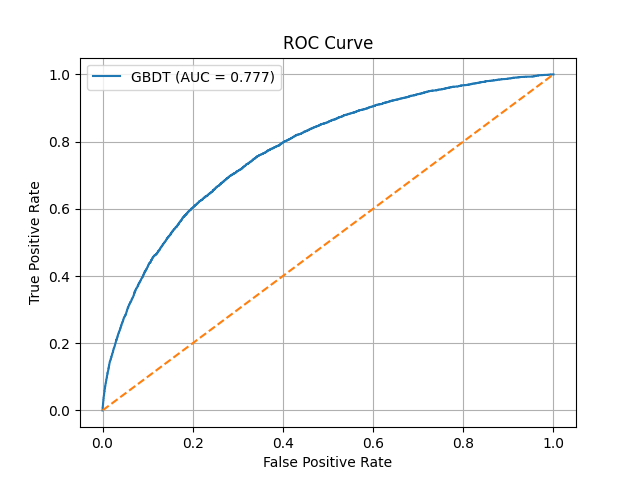
\includegraphics[width=0.65\linewidth]{inc/png/roc_curve.png}
    \end{center}
    \captionsetup{justification=centering}
    \caption{ROC-кривая итоговой модели}
    \label{fig:research_roc_curve}
\end{figure}
\FloatBarrier

ROC-кривая показывает зависимость доли верно выявленных положительных объектов от доли ложноположительных срабатываний при изменении порога классификации. В рассматриваемой задаче положительным классом является дефолт заемщика.

Расположение ROC-кривой выше диагонали случайного классификатора показывает, что модель обладает способностью разделять заемщиков по уровню кредитного риска. Значение ROC-AUC, равное 0.777, подтверждает, что модель выполняет ранжирование заемщиков лучше случайного классификатора.

На рисунке~\ref{fig:research_pr_curve} представлена Precision-Recall кривая итоговой модели.

\FloatBarrier
\begin{figure}[ht!]
    \begin{center}
        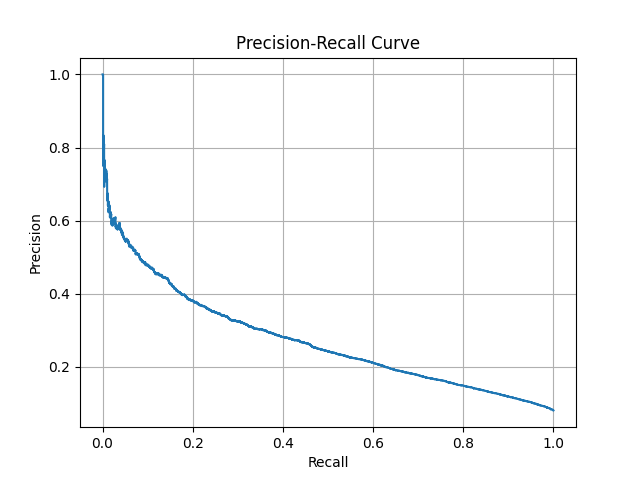
\includegraphics[width=0.65\linewidth]{inc/png/pr_curve.png}
    \end{center}
    \captionsetup{justification=centering}
    \caption{Precision-Recall кривая итоговой модели}
    \label{fig:research_pr_curve}
\end{figure}
\FloatBarrier

Precision-Recall кривая использовалась для оценки качества выявления положительного класса при наличии дисбаланса данных. В отличие от ROC-кривой, данный график позволяет более наглядно оценить работу модели именно для редкого класса, которым в рассматриваемой задаче является дефолт заемщика.

По результатам анализа Precision-Recall кривой можно сделать вывод, что модель обеспечивает высокую полноту выявления дефолтных заемщиков, однако при этом значение точности остается невысоким. Это связано с выбранным порогом классификации 0.3, при котором модель чаще относит заемщиков к группе риска.

Для рассматриваемой задачи кредитного скоринга такой результат является приемлемым. Для банка пропуск дефолтного заемщика может привести к финансовым потерям, тогда как ошибочное отнесение надежного заемщика к группе риска может быть компенсировано дополнительной проверкой заявки.

Таким образом, исследование показало, что выбранный порог классификации соответствует цели снижения кредитного риска за счет повышения полноты выявления потенциально проблемных заемщиков.

\subsection{Выводы}

В ходе исследования были рассмотрены характеристики разработанного программного обеспечения для оценки кредитоспособности физических лиц.

В отличие от функционального тестирования, где проверялась корректность выполнения отдельных сценариев работы приложения, в данном разделе была исследована способность программного комплекса решать основную прикладную задачу — выявлять заемщиков с высоким риском дефолта.

Были определены зафиксированные и варьируемые факторы исследования. К зафиксированным факторам были отнесены набор данных, алгоритм LightGBM, состав входных признаков, структура входных и выходных данных, а также способ взаимодействия приложения с Python-модулем. К варьируемым факторам относятся порог классификации, гиперпараметры модели и характеристики заемщиков.

По результатам исследования установлено, что итоговая модель обеспечивает высокую полноту выявления дефолтных заемщиков. Значение Recall составило 0.89, что свидетельствует о способности модели выявлять большую часть заемщиков с высоким риском дефолта.

Значение ROC-AUC, равное 0.777, показывает, что модель способна разделять заемщиков по уровню кредитного риска лучше случайного классификатора.

Анализ влияния порога классификации показал, что увеличение порога снижает количество ложноположительных решений, однако увеличивает число пропущенных дефолтов. Поэтому для итоговой модели был выбран порог 0.3, позволяющий уменьшить количество пропущенных заемщиков с высоким риском дефолта.

Таким образом, исследование подтвердило применимость разработанного программного обеспечения для предварительной оценки кредитного риска. Разработанное приложение может использоваться как вспомогательный инструмент поддержки принятия решений, при этом окончательное решение о выдаче кредита должно приниматься с учетом дополнительной проверки и экспертной оценки специалиста.